\section{Osnovni pojmi za obravnavo zakonov}

Za natančno formulacijo in razumevanje zakonov moramo uvesti pojem proste grupe.

\subsection{Proste grupe}

Naslednjo definicijo proste grupe najdemo v članku \cite{Pogacnik_2024}.

\begin{definicija}
\label{def_prosta_grupa}
Grupa $F$ je \emph{prosta} nad neprazno množico $S$, če za vsako preslikavo $\iota : S \to F$ in vsako grupo $G$ in vsako preslikavo $\varphi: S \to  G$ obstaja natanko en homomorfizem $\tilde{\varphi} \in \operatorname{Hom}(F, G)$,
da velja $\tilde{\varphi} \circ \iota = \varphi$. Z drugimi besedami, spodnji diagram komutira. Tej lastnosti pravimo \emph{univerzalna lastnost prostih grup}.  
\[ 
\begin{tikzpicture}
    \matrix (m)
      [
        matrix of math nodes,
        row sep    = 3em,
        column sep = 4em
      ]
      {
        S    & G \\
        F  &             \\
      };
    \path
      (m-1-1) edge [{Hooks[right,length=0.8ex]}->] node [left] {$\iota$} (m-2-1)
      (m-1-1.east |- m-1-2)
        edge [->] node [above] {$\varphi$} (m-1-2)
      (m-2-1.east) edge [->,
        dashed] node [right] {$\tilde{\varphi}$} (m-1-2);
  \end{tikzpicture} \]
\end{definicija}

\begin{trditev}
\label{trd_enolicnost_prostih_grup}
 Naj bo $S$ neprazna množica. Potem do izomorfizma natančno obstaja največ ena prosta grupa nad množico $S$.
\end{trditev}
\begin{dokaz}
Dokaz trditve je vzet iz \cite[str.~4]{Pogacnik_2024}.
Naj bosta $F$ in $F'$ prosti grupi nad množico $S$. Označimo z $i$ in $j$ inkluziji $i : S \to F$ in $j : F'$, ki jima po definiciji \ref{def_prosta_grupa} pripadata. Po univerzalni lastnosti prostih grup lahko inkluziji
razširimo do homomorfizmov $\varphi_i : F' \to F$ in $\varphi_j : F \to F'$. 
Kompozitum $\varphi_i \circ \varphi_j : F \to F$ je na množici $S$ identiteta. Ker sta tako $\varphi_i \circ \varphi_j$ kot $\text{id}_F$ razširitvi inkluzije $i$,
mora po enoličnosti razširitev veljati $\varphi_i \circ \varphi_j = \text{id}_F$. Simetrično pokažemo še $\varphi_j \circ \varphi_i  = \text{id}_{F'}$, torej sta grupi $F$ in $F'$ izomorfni.
\[
\begin{tikzpicture}
    \matrix (m1)
      [
        matrix of math nodes,
        row sep    = 3em,
        column sep = 4em
      ]
      {
        S    & F' \\
        F  &             \\
      };
    \path
      (m1-1-1) edge [{Hooks[right,length=0.8ex]}->] node [left] {$i$} (m1-2-1)
      (m1-1-1.east |- m1-1-2)
        edge [->] node [above] {$j$} (m1-1-2)
      (m1-2-1.east) edge [ ->,
        dashed] node [right] {$\varphi_j$} (m1-1-2);
\end{tikzpicture}
\quad
\begin{tikzpicture}
    \matrix (m2)
      [
        matrix of math nodes,
        row sep    = 3em,
        column sep = 4em
      ]
      {
        S    & F' \\
        F  &             \\
      };
    \path
      (m2-1-1) edge [->] node [left] {$i$} (m2-2-1)
      (m2-1-1.east |- m2-1-2)
        edge [{Hooks[right,length=0.8ex]}->] node [above] {$j$} (m2-1-2)
        (m2-1-2) edge [ ->,
        dashed] node [right] {$\varphi_i$} (m2-2-1.east) ;
\end{tikzpicture}\]
\end{dokaz}

Zaradi te trditve je $F(S)$ upravičena oznaka za prosto grupo nad množico $S$. Še več, grupi $F(S)$ in $F(T)$ sta si izomorfni kot grupi natanko tedaj, ko sta si $S$ in $T$ izomorfni kot množici.
Zato bomo v primeru, ko je $S$ končna množica moči $k$, namesto $F(S)$ pisali $F_k$. To grupo imenujemo \emph{prosta grupa ranga $k$}.

Naj bo $S$ poljubna neprazna množica. Definirajmo grupo okrajšanih besed nad množico $S$ kot \begin{equation*}
    S^* := \{ s_1 s_2 \cdots s_n  \vert n \in \mathbb{N}, \forall i = 1, \ldots, n.\,  s_i \in S \cup S^{-1} , \forall i = 1 , \ldots n-1 .\, s_i \neq s_{i + 1}^{-1} \}.
\end{equation*}
Operacija v njej je stikanje besed, ki jim naknadno še okrajšamo sosednje inverze. Ta operacija je dobro definirana, grupa $S^*$ pa prosta nad množico $S$. 
Ti dejstvi sta natančno dokazani v viru \cite[str.~4, trditev 1.9]{Lyndon_Schupp_2015}. Po trditvi \ref{trd_enolicnost_prostih_grup} sledi $S^* \cong F(S)$,
zato si lahko elemente prostih grup predstavljamo kot okrajšane besede. Z upoštevanjem tega dejstva lahko elementom proste grupe $F(S)$ definiramo dolžino.

\begin{definicija}
\label{def_dolzina_besede}
Naj bo beseda $w \in  F(S)$ oblike $w = s_1 \cdots s_n$. Potem število $l(w) := n$ imenujemo \emph{dolžina besede $w$}.
\end{definicija}
\begin{opomba}\label{opm_trikotniska_neenakost}
    Po definiciji množenja besed v prostih grupah je očitno, da za vsaki besedi $w_1 , w_2$ velja trikotniška neenakost $l(w_1 w_2) \le l(w_1) l(w_2)$.
\end{opomba}

Pri konstrukciji zakonov stalno uporabljamo naslednjo na videz očitno trditev, ki jo vendarle moramo dokazati. 

\begin{trditev}\label{trd_prosta_grupa_je_torzijsko_prosta}
    Proste grupe so \emph{torzijsko proste}. Z drugimi besedami, vsi elementi razen enote so neskončnega reda. 
\end{trditev}
\begin{dokaz}
  Dokaz je povzet po \cite[str.~4--5]{Pogacnik_2024}. 
  Naj bo $F(S)$ prosta grupa nad neprazno množico $S$. Recimo, da obstaja beseda $w \in F(S)$ končnega reda oblike $w = a_1 a_2 \ldots a_n$ za paroma neinverzne elemente $a_1, \ldots , a_n \in S$. Naj bo $j : S \to (\mathbb{Z}, +)$ preslikava, ki vse elemente $a_i$ slika v pozitivna števila. Po univerzalni lastnosti prostih grup jo lahko razširimo do homomorfizma $\varphi_j \in \operatorname{Hom}(F(S), \mathbb{Z})$. 
    Ker je $\varphi_j$ homomorfizem, bo $\varphi(w) = \sum_{i = 1}^{n} \varphi(a_i) > 0$. To je prosislovno, saj bi moral red elementa $\varphi(w)$ deliti red besede $w$.
    Grupa $(\mathbb{Z}, +)$ je torzijsko prosta, zato je element $\varphi_j(w)$ v njej neskončnega reda.
\end{dokaz}


Brez dokaza bomo privzeli Nielsen--Schreierjev izrek, ki je klasični rezultat v teoriji prosti grup. Potrebovali ga bomo za dokaz komutatorske leme,
še bolj izrazito pa pri obravnavi zakonov z računalnikom v razdelku \ref{sec_racunalnisko_iskanje}. 

\begin{izrek}[Nielsen--Schreier]
\label{izr_nielsen_schreier}
 Vsaka podgrupa proste grupe je prosta.
\end{izrek}

Bralec lahko dokaz najde v \cite[str.~5--8]{Lyndon_Schupp_2015}.

\subsection{Definicija in osnovne lastnosti zakonov}\label{sec_osnovne_lastnosti_zakonov}

Za začetek uvedimo blago zlorabo notacije. Naj bo podana prosta grupa $F_k = \langle a_1, \ldots, a_k \rangle$ in naj bo $w$ beseda v njej.
Naj bo $G$ grupa in naj bodo $g_1, \ldots, g_k \in G$. Potem definiramo \begin{equation*}
    w(g_1, \ldots, g_k) := \varphi(w),
\end{equation*}
kjer je $\varphi \in \operatorname{Hom}(F_k, G)$ po univerzalni lastnosti induciran s slikami $a_i \mapsto g_i$ za $i = 1, \ldots, k$.
To je formalna definicja intuitivne ideje \glqq vstavljanja konkretnih elementov grupe v abstraktne elemente\grqq~iz uvodnega poglavja. Z njeno pomočjo definiramo zakone.

\begin{definicija}\label{def_zakon_formalna}
    Beseda $w \in F_k$ je \emph{$k$-črkovni zakon v grupi $G$}, če za vse $k$-terice elementov $g_1, \ldots, g_k \in G$ velja $w(g_1, \ldots, g_k) = 1_G$.
    Za vsako podgrupo $H \le G$ pravimo, da je $w \in F_k$ \emph{$k$-črkovni zakon v podgrupi $H$}, če za vse $k$-terice elementov $h_1, \ldots, h_k \in H$ velja $w(h_1, \ldots, h_k) = 1_G$.
\end{definicija}

Ta definicija nam omogoča vpogled v strukturo zakonov. Naj \emph{$K(G, k) \subseteq F_k$ označuje množico $k$-črkovnih zakonov v grupi $G$}. Potem v luči prejšnje definicije velja
\begin{equation*}
K(G, k)  = \bigcap_{\varphi \in \operatorname{Hom}(F_k, G)} \ker(\varphi).   
\end{equation*}  
Ta množica je končni presek edink v $G$ in posledično tudi sama edinka. Še več, je karakteristična, saj za vsak avtomorfizem $\alpha \in \operatorname{Aut}(F_k)$ velja
\begin{equation*}
    K(G, k)  = \bigcap_{\varphi \in \operatorname{Hom}(F_k, G)} \ker(\varphi) = \bigcap_{\varphi \in \operatorname{Hom}(F_k, G)} \ker(\varphi \circ \alpha). 
\end{equation*}  
To je preprosta posledica dejstva, da $\varphi$ preteče grupo $\operatorname{Hom}(F_k, G)$ natanko tedaj, ko jo preteče $\varphi \circ \alpha$.     

\begin{lema}\label{lem_koncni_indeks_koncnega_preseka}
Naj bo $G$ grupa ter $H_1, \ldots, H_n$ njene podgrupe končnega indeksa, torej $[G: H_i] < \infty$ za $i = 1, \ldots, n$. Potem je tudi $\bigcap_{i = 1}^{n} H_i$ podgrupa končnega indeksa v $G$ in velja
\begin{equation*}
\left[ G: \bigcap_{i = 1}^{n} H_i \right]  \le \prod_{i=1}^{n} [G: H_i].  
\end{equation*} 
\end{lema}

\begin{dokaz}
Dovolj je dokazati trditev za $n = 2$, za višje vrednosti sledi z indukcijo. Naj bosta $H_1, H_2 \le G$ podgrupi končnega indeksa, označimo $S: = H_1 \cap H_2$, ki je podgrupa v $G$. Naj bosta $A_1$ in $A_2$ množici odsekov podgrup $H_1$ in $H_2$ v $G$ ter naj bo $A$ množica odsekov podgrupe $S$ v $G$.
 Definiramo preslikavo $f : A \to  A_1 \times A_2$ s predpisom $f(g S ) = (g H_1, g H_2)$. Desna smer sklepa \begin{equation*}
 g S = h S \iff gh^{-1} \in H_1, \, gh^{-1} \in H_2  \iff g H_1 = h H_1, \, g H_2 = h H_2
\end{equation*}  
nam podaja dobro definiranost, leva pa injektivnost preslikave $f$, ki nam podaja oceno $\lvert A \rvert \le  \lvert A_1 \rvert \lvert A_2 \rvert $.    
\end{dokaz}
Z uporabo te leme direktno sledi, da je v primeru končnosti grupe $G$ grupa $K(G, k)$ podgrupa končnega indeksa največ $\lvert G \rvert^{ \lvert G \rvert^k}$ v $F_k$. 
Za vsak homomorfizem $\varphi \in \operatorname{Hom}(F_k, G)$ namreč po prvem izreku o izomorfizmu velja \begin{equation*}
    \lvert F_k / \ker \varphi \rvert = \lvert \operatorname{im} \varphi \rvert \le \lvert G \rvert. 
\end{equation*}
To dejstvo bo še posebej pobmembno pri iskanju zakonov z računalnikom.


\begin{definicija}
\label{def_cayleyev_graf}
Naj bo $G$ grupa in $S \subseteq G$ njena \emph{simetrična} podmnožica. To pomeni, da velja $S = S^{-1} := \{ s^{-1}  \vert s \in S  \}$. Potem $\operatorname{Cay}(G, S)$ označuje graf z vozlišči $V = G$ in povezavami
$E = \left\{ (p, q) \middle|\, p^{-1}q \in  S \right\}$. Imenujemo ga \emph{Cayleyjev graf grupe $G$, generiran z množico $S$}.  
\end{definicija}

\begin{opomba}
Pogoj simetričnosti $S = S^{-1}$ nam pove, da je $\operatorname{Cay}(G, S)$ pravi graf in ne zgolj usmerjeni. Imamo namreč \begin{equation*}
(p,q) \in  E \iff p^{-1}q \in S \iff q^{-1}p \in S \iff (q,p) \in  E.
\end{equation*}  
\end{opomba}

Preden si ogledamo dva primera, dokažimo naslednjo preprosto, a pomembno trditev.

\begin{trditev}\label{trd_lastnosti_cayleyjevega_grafa}
    Naj bo $S$ končna grupa moči $k$. Cayleyjev graf $\text{Cay}(G, S)$ je $\lvert S \rvert$-regularen, povezan graf.
\end{trditev}
\begin{dokaz}
    Naj bo $g \in G$ vozlišče Cayleyjevega grafa $\text{Cay}(G, S)$. Potem je $g$ povezano z enoto $1_G$, saj je $\langle S \rangle = G$, torej lahko zapišemo
    $g = s_1 s_2 \cdots s_n$ za neke elemente $s_i \in S$. Ta produkt določa povezavo v Cayleyjevem grafu. Ker je vsako vozlišče povezano z enoto $1_G$, je graf povezan. Iz $g s_i = g s_j$ sledi $s_i = s_j$, zato iz vsakega vozlišča vodi natanko $\lvert S \rvert$ različnih povezav.
\end{dokaz}

\begin{primer}
Na levi imamo sliko Cayleyjevega grafa diedrske grupe $D_{10} = \langle r, Z \rangle$, generiranega z množico $\{ r, r^4 ,Z \}$. Na desni imamo sliko Cayleyjevega grafa proste grupe $F_2 = \langle a, b \rangle$, generiranega z množico $\{ a^{\pm 1}, b^{\pm 1} \}$. Slika je prosto dostopna na spletu \cite{wikipedia_cayley_graph},
na njej je enota $1_{F_2}$ označena z $e$. Celotnega grafa seveda ne moremo smiselno narisati na sliko, saj so po trditvi \ref{trd_prosta_grupa_je_torzijsko_prosta} proste grupe torzijsko proste, zato imajo neskončno elementov. 
Še več, direktna posledica te trditve je, da je graf na sliki drevo.

\begin{figure}[h]
    \centering
    \begin{minipage}[t]{0.45\textwidth}
        \centering
        \tikzset{vertex/.style={draw, thick, circle, fill=orange!50, minimum size=20pt, inner sep=0pt}}
        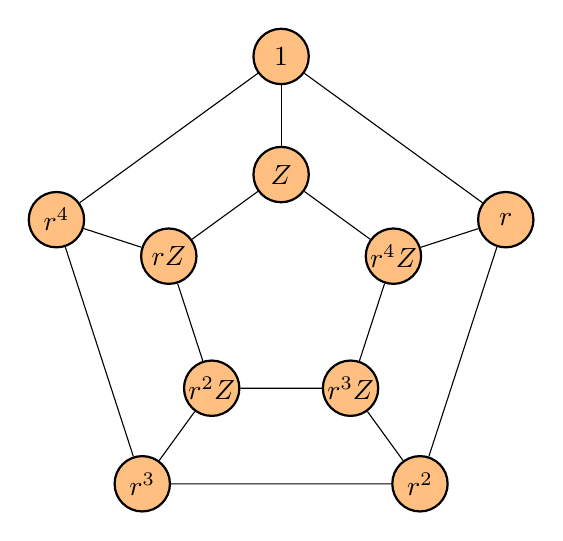
\begin{tikzpicture}[rotate=90, scale=1.5]
            \node[vertex] (v1) at (-0*360/5:1) {$Z$};
            \node[vertex] (v2) at (-0*360/5:2) {$1$};
            \node[vertex] (v3) at (-1*360/5:1) {$r^4Z$};
            \node[vertex] (v4) at (-1*360/5:2) {$r$};
            \node[vertex] (v5) at (-2*360/5:1) {$r^3Z$};
            \node[vertex] (v6) at (-2*360/5:2) {$r^2$};
            \node[vertex] (v7) at (-3*360/5:1) {$r^2Z$};
            \node[vertex] (v8) at (-3*360/5:2) {$r^3$};
            \node[vertex] (v9) at (-4*360/5:1) {$rZ$};
            \node[vertex] (v10) at (-4*360/5:2) {$r^4$};
            
            \draw (v1) -- (v2);
            \draw (v1) -- (v3);
            \draw (v2) -- (v4);
            \draw (v3) -- (v4);
            \draw (v3) -- (v5);
            \draw (v4) -- (v6);
            \draw (v5) -- (v6);
            \draw (v5) -- (v7);
            \draw (v6) -- (v8);
            \draw (v7) -- (v8);
            \draw (v1) -- (v9);
            \draw (v7) -- (v9);
            \draw (v2) -- (v10);
            \draw (v8) -- (v10);
            \draw (v9) -- (v10);
        \end{tikzpicture}
        \caption{Graf $\text{Cay}(D_{10}, \{ r, r^4 , Z \})$.}
    \end{minipage}%
    \hspace{0.05\textwidth}
    \begin{minipage}[t]{0.45\textwidth}
        \centering
        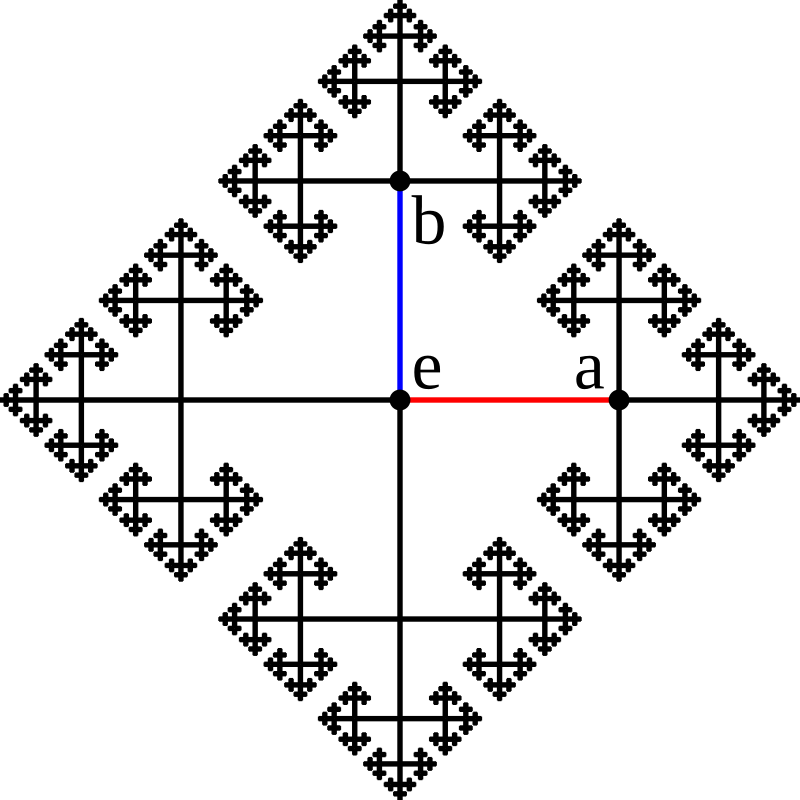
\includegraphics[width=\textwidth]{Cayley_graph_of_F2.svg.png} % Replace with your image file
        \caption{Graf $\text{Cay}(F_2, \{ a^{\pm 1}, b^{\pm 1} \})$.}
    \end{minipage}
\end{figure}


    % \begin{figure}[h]
    %     \centering
    %     \begin{minipage}{0.45\textwidth}
    %         \centering
    %         \tikzset{vertex/.style={draw, thick, circle, fill=orange!50, minimum size=20pt, inner sep=0pt}}
    % \begin{tikzpicture}[rotate=90, scale=1.5]
    % \node[vertex] (v1) at (-0*360/5:1) {$Z$};
    % \node[vertex] (v2) at (-0*360/5:2) {$1$};
    % \node[vertex] (v3) at (-1*360/5:1) {$r^4Z$};
    % \node[vertex] (v4) at (-1*360/5:2) {$r$};
    % \node[vertex] (v5) at (-2*360/5:1) {$r^3Z$};
    % \node[vertex] (v6) at (-2*360/5:2) {$r^2$};
    % \node[vertex] (v7) at (-3*360/5:1) {$r^2Z$};
    % \node[vertex] (v8) at (-3*360/5:2) {$r^3$};
    % \node[vertex] (v9) at (-4*360/5:1) {$rZ$};
    % \node[vertex] (v10) at (-4*360/5:2) {$r^4$};
    
    % \draw (v1) -- (v2);
    % \draw (v1) -- (v3);
    % \draw (v2) -- (v4);
    % \draw (v3) -- (v4);
    % \draw (v3) -- (v5);
    % \draw (v4) -- (v6);
    % \draw (v5) -- (v6);
    % \draw (v5) -- (v7);
    % \draw (v6) -- (v8);
    % \draw (v7) -- (v8);
    % \draw (v1) -- (v9);
    % \draw (v7) -- (v9);
    % \draw (v2) -- (v10);
    % \draw (v8) -- (v10);
    % \draw (v9) -- (v10);
    % \end{tikzpicture}
    %         \caption{Your TikZ diagram caption}
    %     \end{minipage}%
    %     \hspace{0.05\textwidth}
    %     \begin{minipage}{0.45\textwidth}
    %         \centering
    %         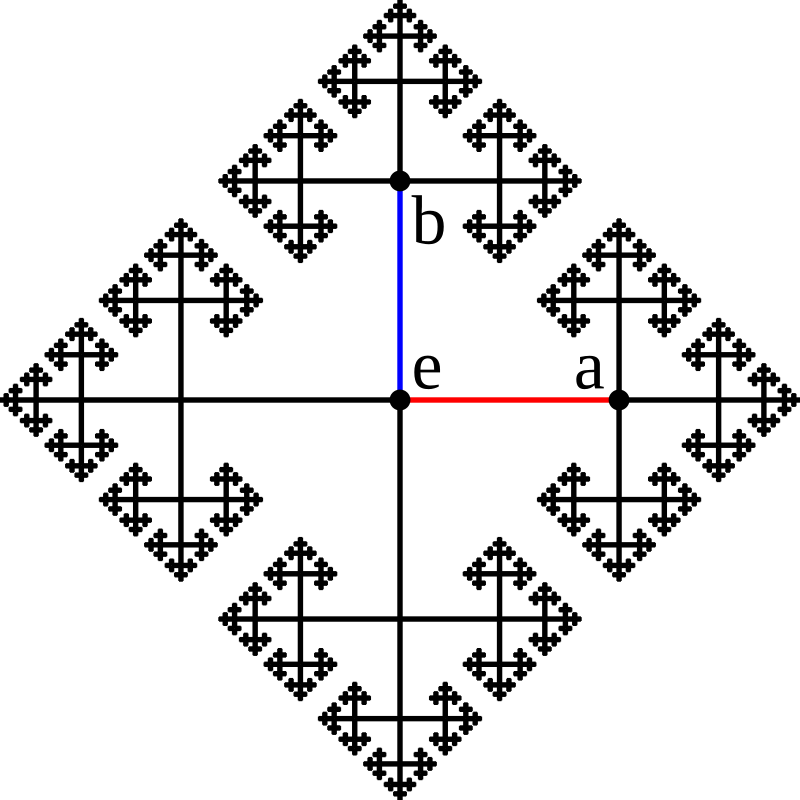
\includegraphics[width=\textwidth]{Cayley_graph_of_F2.svg} % Replace with your image file
    %         \caption{Your figure caption}
    %     \end{minipage}
    % \end{figure}

\end{primer}

\begin{definicija}\label{def_ozina}
    Številu \begin{equation*}
    \operatorname{\alpha}_{k}(G) := \min \left\{ l(w)  \middle|\,  w \in F_k \setminus \left\{ 1\right\} \text{ je zakon v } G  \right\} \cup \left\{ \infty\right\} 
    \end{equation*}  
    rečemo \emph{$k$-črkovna ožina grupe $G$}.  
    \end{definicija}
    

\begin{opomba} % TODO tole malo popravi, ni čisto logično ubesedeno
Ime ožina grupe -- ki je uporabljeno na primer v virih \cite{Schneider_2016}, \cite{Bradford_Thom_2017} in \cite{Schleimer_2001} -- je nekoliko zavajajoče. Izhaja iz Cayleyjevega grafa grupe, vsak njegov cikel $g_1 , g_2, \ldots, g_n, g_1$ namreč
podaja zvezo $s_1 s_2 \cdots s_n = 1_G$ za elemente $s_i \in S$, kjer za $i = 2, \ldots, n$ velja $s_i = g_{i - 1}^{-1} g_i$ in $s_1 = g_n^{-1} g_1$.
V kontekstu zakonov je to ime do neke mere neupravičeno, saj beseda $s_1 s_2 \cdots s_n$ ni nujno zakon v grupi. Če si pogledamo na primer grupo $C_3 \times C_5 = \langle (\xi, 1), (1, \eta) \rangle$,
bo Cayleyjev graf $\text{Cay}(C_3 \times C_5, \{ (\xi, 1)^{\pm 1} , (1, \eta)^{\pm 1} \})$ vseboval 3-cikel, ki ga porodi generator $(\xi , 1)$. Po drugi strani pa beseda $\xi^3$ očitno ni zakon v grupi $C_3 \times C_5$, ki premore element reda 5.
Ker je grupa $C_3 \times C_5$ Abelova, ni težko razmisliti, da velja $\alpha_k(C_3 \times C_5) = 4$ za $k \ge 2$ in $\alpha_1(C_3 \times C_5) = 15$. 

\end{opomba}

Izkaže se, da so najbolj zanimivi in za obravnavo relevantni dvočrkovni zakoni. To nam sporočata naslednji dve trditvi.
\begin{trditev}
\label{trd_vlozitev_proste_grupe}
 Obstaja vložitev grupe $F_{2 \cdot 3^{k}} = \langle a_1, \ldots, a_{2 \cdot 3^{k}} \rangle$ v grupo $F_2 = \langle a,b \rangle $, tako da velja $l(a_i) = 2k + 1$. Tu smo z $l(w)$ označili dolžino besede $w \in F_2 = \langle a,b \rangle$. 
\end{trditev}


\begin{dokaz}
Dokaz trditve ni posebno zahteven, vendar je nekoliko preveč tehničen za naše potrebe, saj bi zahteval uvedbo in razumevanje pojmov Schreierjevega grafa ter fundamentalne grupe grafa, ki ju tekom naloge sicer ne potrebujemo. Naveden je v~\cite[str.~5]{Schneider_2016}, glavna ideja je obravnavati Cayleyev graf proste grupe $F_2$ z dvema generatorjema.
Drevo vseh besed dolžine $k$ na ustrezen način dopolnimo (do Schreierjevega grafa) tako, da dodamo povezave listom. Pri tem dobimo cikle dolžine $2k + 1$ in (s pomočjo fundamentalne grupe grafa) utemeljimo, da lahko jih lahko obravnavamo kot elemente $F_{2 \cdot 3^{k}}$, vložene v $F_2$. 
\end{dokaz}


\begin{posledica}\label{psl_veccrkovni_zakoni_meje}
Naj bo $G$ grupa in $k \ge 2$ naravno število. Potem velja \begin{equation*}
     \alpha_k(G) \le  \alpha_2(G) 
\end{equation*}  
in \begin{equation*}
\alpha_2(G) \le \left( {2 \left\lceil \log_3 \left(\frac{k}{2} \right) \right\rceil + 1  } \right) \alpha_k(G).
\end{equation*}  
\end{posledica}
\begin{dokaz}
    Prva neenakost je očitna, saj so vsi dvočrkovni zakoni tudi $k$-črkovni zakoni. Druga neenakost drži, saj lahko po prejšnji trditvi vložimo $F_{{2 \left\lceil \log_3(\frac{k}{2}) \right\rceil}}$ v $F_2$
    tako, da noben generator ni daljši od ${2 \left\lceil \log_3(\frac{k}{2}) \right\rceil + 1  }$. Hkrati velja $F_k \subseteq F_{{2 \left\lceil \log_3(\frac{k}{2}) \right\rceil}}$, kar nam da želeno neenakost.
\end{dokaz}


\subsection{Teorija naključnih sprehodov}

Za obravnavo zakonov v simetričnih grupah bomo potrebovali naključne sprehode, natančneje lene naključne sprehode.
Tekom razdelka naj bo $G$ grupa, generirana s simetrično podmnožico $S \subseteq G$. Poleg tega naj bo $\Gamma := \operatorname{Cay}(G, S)$, ki je po trditvi \ref{trd_lastnosti_cayleyjevega_grafa}
regularni povezani graf, kar nam nekoliko poenostavi potrebno teoretično ozadje o naključnih sprehodih.

\begin{definicija}
\label{def_leni_nakljucni_sprehod}
    \emph{Leni naključni sprehod} je naključno zaporedje elementov $s_n \in S$ za $n \in \mathbb{N} \cup \left\{ 0\right\} $, porojeno s formulo \begin{equation*}
        \mathbb{P}(s_{n+1} = g   \vert \,  s_n = h) = \begin{cases}
            \frac{1}{2}; & \text{če }  g = h, \\
            \frac{1}{2 \lvert S \rvert }; & \text{če } g = sh \text{ za neki } s \in S.
        \end{cases}
    \end{equation*}
    Tak naključni sprehod nam porodi zaporedje besed $w_n := s_0 s_1 \cdots s_n$.  
\end{definicija}
Na vsakem koraku lenega naključnega sprehoda se torej z verjetnostjo $1 / 2$ element ne spremeni, z verjetnostjo $1 / 2$ pa se naključno spremeni v enega od svojih sosedov, ki jih je $\lvert S \rvert$.
To lahko opišemo tudi z matrikami. Za začetek označimo elemente grupe $G$ z $g_1 := 1_G, g_2 , \ldots, g_{\lvert G \rvert}$. Naj bo $u_n$ $\lvert G \rvert$-razsežni vektor, ki predstavlja verjetnostno porazdelitev elementa $s_n$. Z drugimi besedami, $i$-ta komponenta vektorja $u_n$ nam pove verjetnost, da se naključni sprehod po $n$-korakih nahaja v elementu $g_i$. Naj se ta naključni sprehod začne v enoti grupe $G$, kar zapišemo kot $u_0 := (1, 0, \ldots , 0)^T$. 
Zdaj definiramo \emph{matriko lenega naključnega sprehoda} $M \in M_{\lvert G \rvert }(\mathbb{R})$, s predpisom    
\begin{equation*}
M = \frac{1}{2} \left(I + \frac{1}{\lvert S \rvert } A \right) = \frac{1}{2} \left(I + \tilde{A} \right),
\end{equation*}  
kjer smo z $A$ označili matriko soseščine grafa $\Gamma$, z $\tilde{A}$ pa smo označili matriko $\frac{1}{\lvert S \rvert} A$. Ni težko premisliti, da po definiciji \ref{def_leni_nakljucni_sprehod} sledi zveza 
\begin{equation*}
u_n = M^{n} u_0,
\end{equation*}  
ki nam omogoča vpogled v lastnosti naključnih sprehodov. 

\begin{lema}
\label{lem_M_je_sebiadjungirana}
Matrika $M$ je diagonalizabilna, sebiadjungirana in njene lastne vrednosti ležijo v intervalu $[0, 1]$.
\end{lema}
\begin{dokaz}
Ker je realna matrika $M$ simetrična, je diagonalizabilna, sebiadjungirana in velja, da so vektorji, ki pripadajo paroma različnim lastnim vrednostim, med seboj ortogonalni. Enako velja za matriko $A$. Sebiadjungiranost nam implicira realnost lastnih vrednosti matrik $M$ in $A$.
Z oceno matričnih norm \begin{equation*}
    \sqrt{ \lambda_{\max} \left(\tilde{A}^2\right)} = \sqrt{\lambda_{\max} \left(\tilde{A}^{T} \tilde{A} \right)}  = \lvert\lvert \tilde{A} \rvert\rvert_2 \le \sqrt{\lvert\lvert A \rvert\rvert_1 \lvert\lvert \tilde{A} \rvert\rvert_{\infty}} = 1 
\end{equation*}  
sledi, da ima matrika $\tilde{A}$ lastne vrednosti v intervalu $[-1 ,1]$, kar pomeni, da lastne vrednosti matrike $M$ ležijo v intevalu $[0, 1]$. 
\end{dokaz}

Ker vemo, da so vse lastne vrednosti realne, jih lahko po razvrstimo po velikosti: 
\begin{equation*}
1 \ge \lambda_1(G, S) \ge \lambda_2(G, S) \ge \ldots \ge \lambda_{\lvert G \rvert }(G, S) \ge 0.  
\end{equation*}  
Ker je $\Gamma$ povezan graf, velja $\lambda_1(G, S) = 1 > \lambda_2(G, S)$, lastni vektor vrednosti $\lambda_1(G, S)$ pa pripada enakomerni porazdelitvi $u := 1/ \lvert G \rvert (1, \ldots, 1)^T$. Ti dejstvi sta natančneje dokazani v \cite{Milanez_2022},
intuitivno pa je jasno, da vsaj ena lastna vrednost mora biti enaka $1$, saj mora biti vsota komponent vektorjev $u_n = M^n u_0$ vedno enaka $1$.

Razliko $1 - \lambda_2(G, 2)$ imenujemo \emph{spektralna razlika} grafa $\Gamma$. 

\begin{definicija}
\label{def_diameter_cayleyjevega_grafa}
Naj bo $G$ končna grupa.
\emph{Diameter Cayleyjevega grafa} \\ $\Gamma = \operatorname{Cay}(G, S)$ je število \begin{equation*}
    \operatorname{diam}(G, S) := \min \left\{ n \in \mathbb{N}  \middle|\, \forall g \in G. \exists s_1, \ldots , s_n \in S \cup \left\{ 1_G \right\} . g = s_1 \cdots s_n \right\}.
\end{equation*}  
\end{definicija}
Intuitivno nam diameter Cayleyjevega grafa poda najmanjše število korakov, po katerem lahko naključni sprehod po grafu $\Gamma$ doseže poljubni element grupe $G$.
Za ocenjevanje dolžin zakonov v grafih je bistvena sledeča zveza med diametrom grafa in spektralno razliko lenega naključnega sprehoda.

\begin{trditev}
\label{trd_zveza_med_diametrom_grafa_in_spektralno_razliko}
 Velja zveza \begin{equation*}
 1 - \lambda_1(G, S) \ge \frac{1}{2 \lvert S \rvert \operatorname{diam}(G, S)^2}.
 \end{equation*}  
\end{trditev}
\begin{dokaz}
Dokaz najdemo v \cite{Diaconis_1993} kot posledico 1.  % TODO najdi referenco za dokaz te leme, oz si poglej vir, na katerega se sliče Thom
\end{dokaz}

Od tod sledi pomembna posledica. \begin{posledica}
\label{psl_posledica_zveze_diameter}
Naj bo vektor $u := \frac{1}{\lvert G \rvert} (1, \ldots, 1)^T$ in naj bo $u_0 := (1, 0, \ldots ,0)^T$. Potem velja ocena \begin{equation*}
\lvert \lvert M^{n} u_0 - u \rvert \rvert_2 \le \lambda_2(G, S)^{n} \le \left( 1 - \frac{1}{2 \lvert S \rvert \operatorname{diam}(G, S)^2 } \right)^{n} \le \exp(- \frac{n}{2 \lvert S \rvert \text{diam}(G, S)^2 }). 
\end{equation*}    
\end{posledica}
\begin{dokaz}
Srednja neenakost je direktna posledica trditve \ref{trd_zveza_med_diametrom_grafa_in_spektralno_razliko}. Desna je posledica Bernoullijeve nenakosti $1 - x \le \exp(-x)$, ki velja za vsa pozitivna realna števila $x$.
Leva neenakost pa nam sporoča, da vektor $u_n$ konvergira proti enakomerni porazdelitvi $u$. Ideja za dokaz je vzeta iz \cite[str.~2]{Trevisan_2008} in poteka tako, da lastnim vrednostim $\lambda_i(G, S)$ priredimo njihove paroma ortogonalne lastne vektorje $v_i(G, S)$.
Potem dobimo \begin{align*}
  \left|\left| M^{n}u_0 -  u  \right|\right|_2 &= \left|\left|  \sum_{i = 2}^{\left| G \right|} \lambda_i(G, S)^n  v_i(G, S)     \right|\right|_2  \\
    &= \sqrt{ \sum_{i = 2}^{\left| G \right|} \lambda_i(G, S)^{2n}  \left| v_i(G, S) \right|^2   }  \\
    &\le \max_{i = 2, \ldots, \left| G \right| } \left| \lambda_i \right|^{n} \sqrt{\sum_{i = 2}^{\left| G \right| } \left| v_i(G, S) \right|^2} \\
    &\le   \max_{i = 2, \ldots, \left| G \right| } \left| \lambda_i(G, S) \right|^{n} \left|\left| u \right|\right|_2 \\
    &\le \lambda_2(G, S)^{n} \lvert\lvert u \rvert\rvert_1 \\
    &= \lambda_2(G, S)^{n}.
\end{align*}
\end{dokaz}

Za konec potrebujemo še zadnjo lemo, ki je podana kot trditev 3.1 v \cite{Kozma_Thom_2016}. 
\begin{lema}\label{lem_posledica_neenakosti_csb}
Naj bo $E$ podmnožica grupe $G$ in naj bo $\alpha := \lvert E \rvert / \lvert G \rvert$ in naj bo $(w_n)_{n \in  \mathbb{N}}$ leni naključni sprehod.
Če velja ocena \begin{equation*}
n \ge 2 \lvert S \rvert \operatorname{diam}(G, S)^2 \log(2 \lvert G \rvert ), 
\end{equation*}  
    velja $\mathbb{P}(w_n \in E) \ge \alpha / 2$.
\end{lema}  
\begin{dokaz}
Po predpostavki velja ocena \begin{equation*}
  \left( 1 - \frac{1}{2 \lvert S \rvert \operatorname{diam}(G, S)^2 } \right)^{n} \le \exp(- \frac{n}{2 \lvert S \rvert \text{diam}(G, S)^2 } \le \frac{1}{2 \lvert G \rvert}.
\end{equation*}
Nato definrajmo vektor $\chi_E = 1 / G (h_1 , \ldots , h_{\lvert G \rvert })$, kjer so za vsak $ i = 1, \ldots, \lvert G \rvert $ \begin{equation*}
  h_i := \begin{cases}
      1; & \text{če } g_i \in E, \\
      0; & \text{če } g_i \not\in E.
  \end{cases}
\end{equation*}
Potem sledi sklep \begin{align*}
    \mathbb{P}(s_n \in E) &= \langle u_n , \chi_E \rangle  \\
     &\ge \langle u, \chi_E \rangle -  \left( 1 - \frac{1}{2 \lvert S \rvert \operatorname{diam}(G, S)^2 } \right)^{n} \lvert\lvert \chi_E \rvert\rvert \\
     &= \frac{\lvert E \rvert }{\lvert G \rvert } - \left( 1 - \frac{1}{2 \lvert S \rvert \operatorname{diam}(G, S)^2 } \right)^{n} \sqrt{E} \\
     &\ge  \frac{\lvert E \rvert }{\lvert G \rvert } - \frac{\sqrt{E}}{2 \lvert G \rvert } \\
     &\ge \frac{\lvert E \rvert }{2 \lvert G \rvert } \\
     &=  \alpha / 2.
\end{align*} 
\end{dokaz}

Ta ocena nam bo pomagala pri dokazu obstoja kratkih zakonov v simetričnih grupah.
Glavni rezultat, ki bo zagotovil ta preboj, je Helfgott--Seressov izrek, ki omeji diameter Cayleyjevih grafov simetričnih grup, generiranih s parom elementov. \begin{izrek}[Helfgott--Seress]\label{izr_Helfgott_Seress}
Naj par $(\sigma, \tau) \in S_n^2$ generira grupo $S_n$, torej $\langle \sigma, \tau \rangle = S_n$. Potem obstaja konstanta $C > 0$, da je diameter grafa $\Gamma = \operatorname{Cay}(S_n, \left\{ \sigma^{\pm 1}, \tau^{\pm 1} \right\} )$ največ 
\begin{equation*}
\exp(C \log(n)^{4} \log(\log(n))).
\end{equation*}
\end{izrek}  
Dokaz tega izreka je zelo težek in se močno zanaša na klasifikacijo končnih enostavnih grup, zato ga opuščamo. Bralec ga lahko najde v članku \cite{Helfgott_Seress_2013}.
